Le analisi relative al parametro $\gamma$ sono state effettuate in maniera analoga a quelle precedenti: per ogni valore d'interesse di $\gamma$ sono state effettuate 10 simulazioni ognuna delle quali mantenendo invariati tutti gli altri parametri.
In particolare, le dimensioni della mappa sono state mantenute pari a 30$\times$30 celle, sono stati impiegati 6 robot con un raggio di visione pari a 6 celle, come suggerito dal processo di ottimizzazione descritto nel Capitolo \ref{chap:pso}, un raggio del ripetitore pari a 3 celle e abilitando i feriti a poter segnalare le loro posizioni.
Per quanto riguarda le mappe, sono state sfruttate le 5 mappe generate casualmente e utilizzate per le analisi condotte sul parametro $\alpha$ (Sezione \ref{sec:alpha}).
Infine, poiché ci si è accorti che il valore di $\alpha$ sia in grado di influenzare la distanza che mantengono tra loro i robot, si è deciso di effettuare due batterie di test: una prima in cui si è mantenuto un valore di $\alpha$ basso pari a $10^{-4}$ e poi per uno elevato pari a 8.175 (valore consigliato dal processo di ottimizzazione).
Le due batterie di test sono state eseguite in modo separato e autonomamente l'una dall'altra, non modificando altri parametri (escluso $\gamma$).\\
La metrica utilizzata per valutare come il parametro influisce nel comportamento del modello è stata la distanza media tra i robot. Come già detto, ci si aspetta che per valori alti di $\gamma$ gli agenti tendano a tenersi più distanti tra loro e viceversa.
Formalmente, la metrica viene computata nel seguente modo: per ogni robot si è calcolata la media delle distanze euclidee tra l'agente di interesse e tutti gli altri robot; in seguito, si è computata la media (e relativa deviazione standard) delle distanze medie.
Tale metrica è stata misurata ad ogni \textit{step} della simulazione.
Di seguito, mostriamo i principali risultati ottenuti in entrambe le batterie di test, ulteriori dati prodotti, meno significativi, sono riportati in Appendice \ref{apx:gamma}.

\subsection{Analisi con valore di $\alpha$ basso}
\label{subsec:gammaalow}
Una prima analisi effettuata è stata considerare per ogni valore del parametro la distribuzione della distanza media, ovvero in quanti \textit{step} si è presentato un determinato valore di distanza media; tali distribuzioni sono state calcolando aggregando i dati di tutte le simulazioni per ogni valore del parametro.
In Figura \ref{fig:gammaDistr} sono mostrate le distribuzioni per due valori di $\gamma$ (le altre sono riportate in Appendice \ref{apx:gamma}); si noti che la scala sull'asse delle \textit{y} è logaritmica e la distribuzione è rappresentata solo da un \textit{marker} che indica il numero di \textit{step} in cui si è verificate quel valore di distanza. Si tenga inoltre presente che i valori di distanza sono stati raggruppati per numeri interi.
Nelle distribuzioni mostrate, si nota come che per un valore di $\gamma$ pari a 0.32 (Figura \ref{sfig:gammaDistr0.32}), gli agenti tendano a mantenere una distanza nell'“intorno” di 30, con pochi casi di distanze pari o superiori a 50; al contempo, con un valore pari a 0.65 (Figura \ref{sfig:gammaDistr0.65}), si nota come non vi sia un valore di distanza che viene assunto significativamente più frequentemente di altri, ma il grafico presenta una distribuzione più “liscia”.\\
\begin{figure}
	\subfloat[Distribuzione della distanza media mantenuta dai robot con un valore di $\gamma$ pari a 0.32.\label{sfig:gammaDistr0.32}]{
		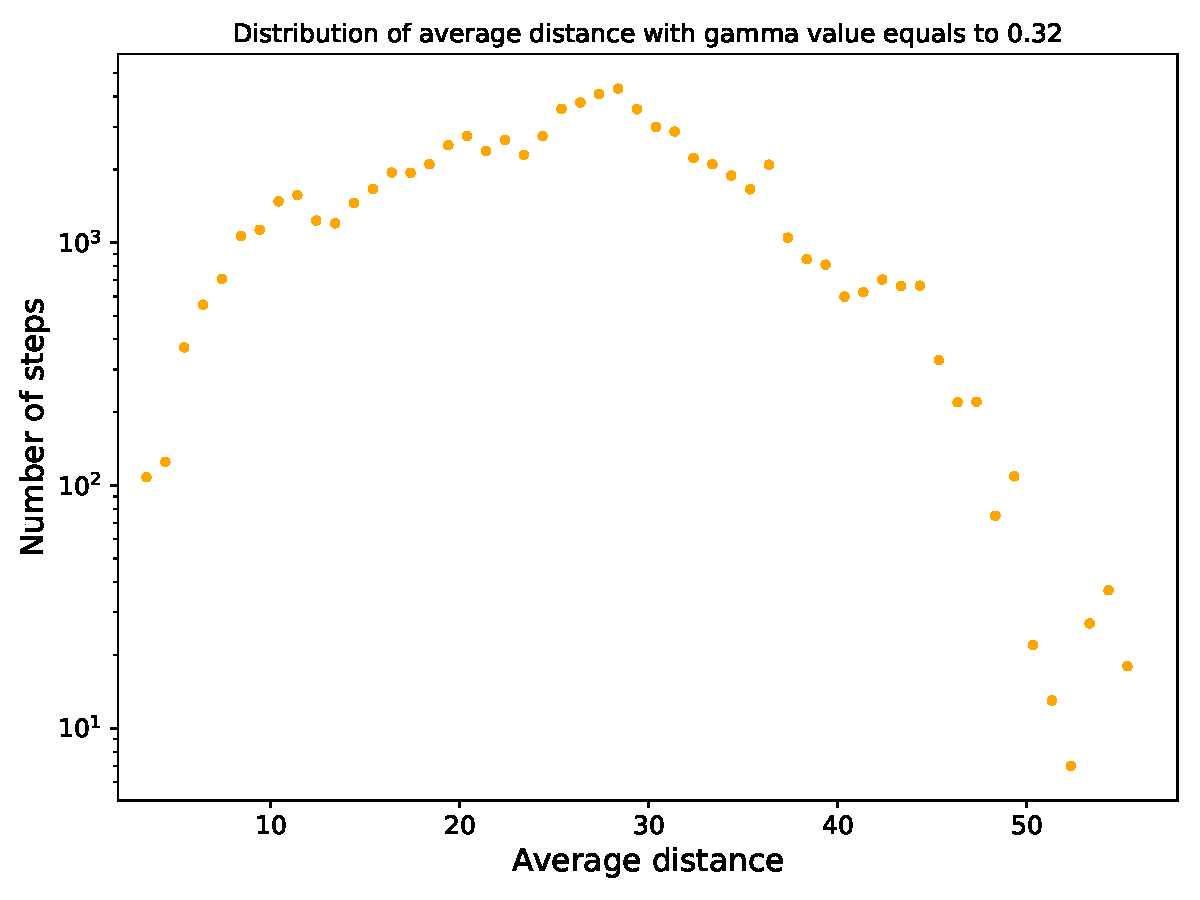
\includegraphics[width=.47\linewidth]{images/gamma_results/low_alpha/distribution_distance_gamma_0_32}
	}
	\hfill
	\subfloat[Distribuzione della distanza media mantenuta dai robot con un valore di $\gamma$ pari a 0.65.\label{sfig:gammaDistr0.65}]{
		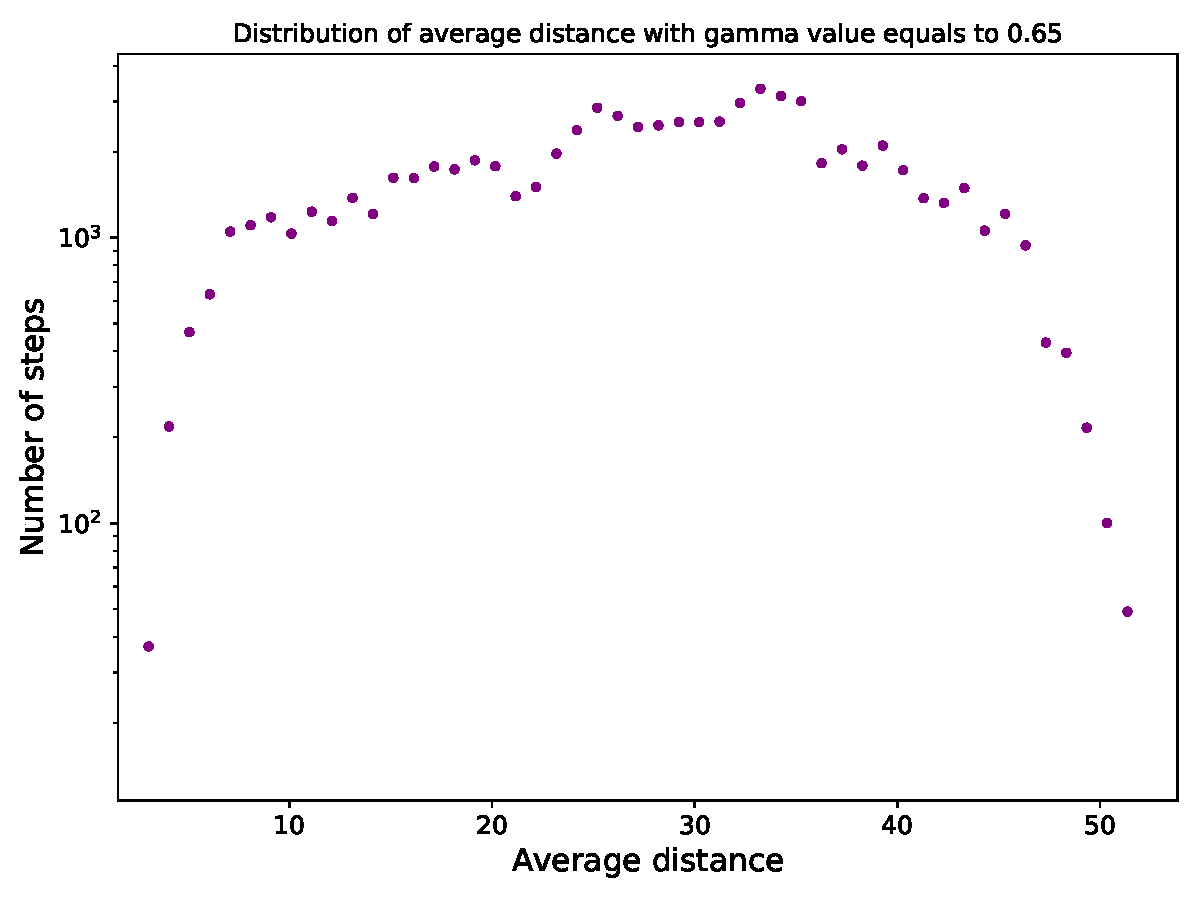
\includegraphics[width=.47\linewidth]{images/gamma_results/low_alpha/distribution_distance_gamma_0_65}
	}
	\caption{Distribuzione della distanza media mantenuta dai robot al variare del valore di $\gamma$, per valutare la distribuzione si è conteggiato in quanti \textit{step} i robot hanno presentato tale distanza, il numero di \textit{bin} per produrre la distribuzione è pari alla differenza tra la distanza minima e massima presente durante la simulazione, tale valore è stato poi arrotondato. Infine si noti che l'asse delle \textit{y} è a scala logaritmica.}
	\label{fig:gammaDistr}
\end{figure}
Poiché effettuare dei confronti solo mediante grafici di distribuzioni realizzati ognuno per ogni valore analizzato di $\gamma$ risulta complicato e poco significativo, si è deciso di confrontarli unendo tali distribuzioni nello stesso grafico; si noti che l'asse delle \textit{y} non è più a scala logaritmica, in modo da favorire un confronto qualitativo delle distribuzioni.
Il grafico complessivo, riportato in Figura \ref{fig:gammaComparison}, mostra come al crescere de valore $\gamma$ la distanza media tra gli agenti tende ad aumentare per un numero maggiore di \textit{step}.
In particolare si può notare come che per valori di $\gamma$ pari a 0.32 e 1 si presentino dei veri e propri “picchi”; è interessante che per il valore pari a 0.65 non vi sia un vero e proprio “picco” ma, come già detto, la distribuzione risulti più “liscia”, presentando al contempo un numero maggiore di \textit{step} con distanze medie tra 40 e 50 (che risultano essere distanze elevate) e che non compaiono in modo così significativo per nessun altro valore di $\gamma$.
Per valori bassi di $\gamma$ non si evidenziano significative differenze in termini di distanza, ma comunque tende ad emergere una concentrazione di valori di distanza relativamente bassi rispetto agli altri valori di $\gamma$.
In particolare, valutando con attenzione la Formula \ref{math:utility-red} grazie a cui l'utilità di una cella viene ridotta, possiamo intuire che un valore basso di $\gamma$ porta tutte le celle percepite dal robot ad avere un'utilità molto simile e prossima allo $0$. Viceversa, un valore alto di $\gamma$ genera una netta differenza tra celle immediatamente circostanti alla posizione e celle più lontane, garantendo un'efficace meccanismo di dissuasione per gli altri robot.\\
Riassumendo quanto valutato fin'ora, si nota come con un valore di $\alpha$ basso, il parametro $\gamma$ influenza la distanza tra gli agenti, presentando un comportamento particolare per il valore di $\gamma$ pari a 0.65 che è stato quello suggerito dal processo di ottimizzazione (si faccia riferimento al Capitolo \ref{chap:pso}).
\begin{figure}
	\centering
	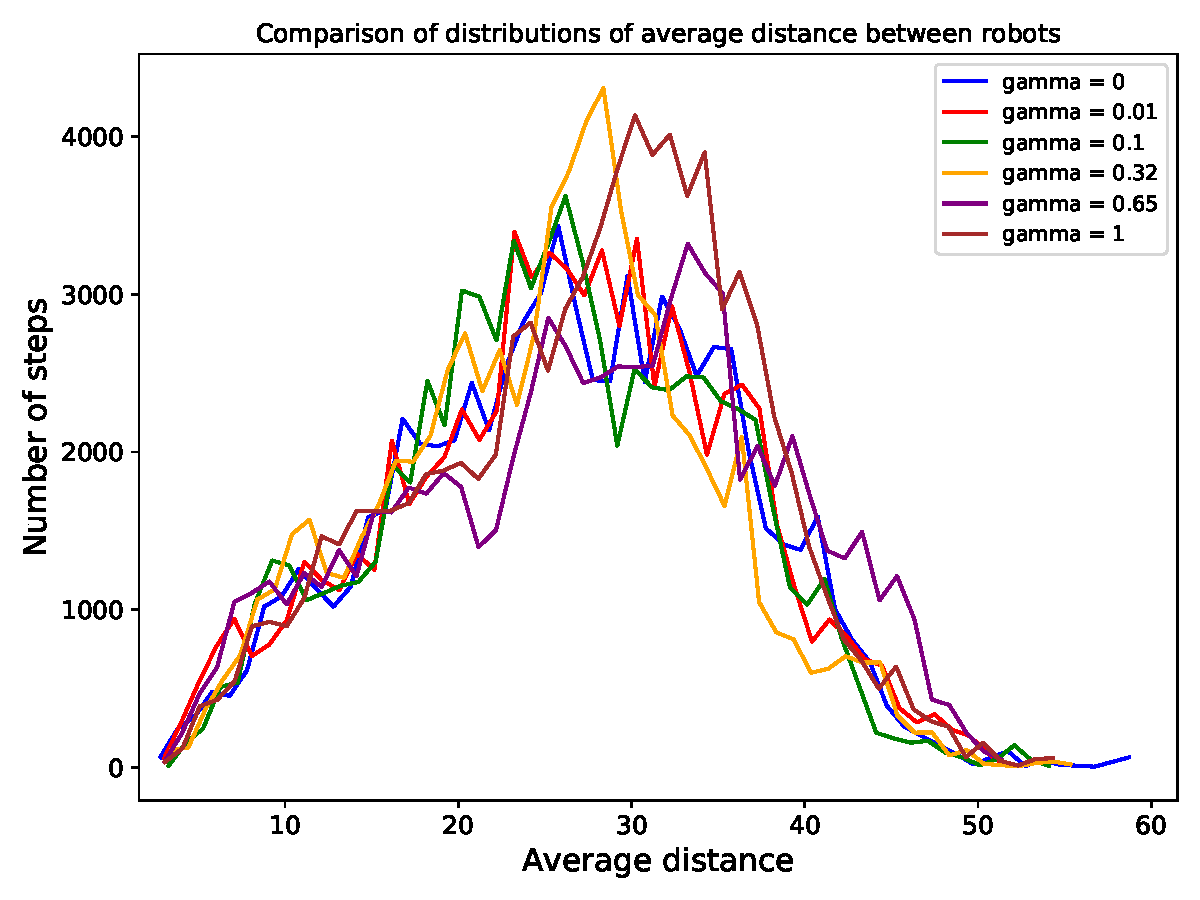
\includegraphics[width=0.9\linewidth]{images/gamma_results/low_alpha/comparison}
	\caption{Grafico che riassume tutte le distribuzioni di distanze medie durante le simulazioni per ogni valore di $\gamma$, si noti che l'asse delle \textit{y} non è più logaritmico.}
	\label{fig:gammaComparison}
\end{figure}

Infine, \margin{Come $\alpha$ influenza la distanza tra gli agenti}si è andati a studiare l'evolversi all'interno della singola simulazione (ne è stata scelta una casualmente tra le dieci eseguite per ogni valore di $\gamma$ studiato) della distanza media tra i robot.
Tali evoluzioni sono mostrate in Figura \ref{fig:gammaSim} per quanto riguarda i valori del parametro pari a 0.32 (Figura \ref{sfig:gammaSim0.32}) e 0.65 (Figura \ref{sfig:gammaSim0.65}), per gli altri si faccia riferimento all'Appendice \ref{apx:gamma}.
In entrambe le simulazioni emerge come più di una volta la distanza tra gli agenti sia diminuita drasticamente e repentinamente per poi, dopo pochi \textit{step}, ricominciare ad aumentare.
Si è associato tale fenomeno alla possibilità da parte dei feriti di segnalarsi, in particolare, ogni volta che qualcuno si segnala, la priorità delle celle del vicinato viene incrementata, e quindi incrementa l'\textit{info-gain} di tali celle.
Notiamo però che questo fenomeno sembra essere meno presente mano a mano che gamma cresce: questo è probabilmente dovuto al fatto che, al crescere di gamma, l'utilità delle celle nell'intorno di una cella che viene esplorata è fortemente diminuito, mentre le celle più distanti subiscono meno questo malus. Nella scelta della cella bersaglio, essendo $\alpha$ molto basso, la differenza tra utilità e priorità di una cella potrebbe propendere verso la prima componente, rendendo quindi una cella proritizzata vicina a una cella già esplorata meno interessante di una priva di priorità ma più distante.
Poiché il valore di $\alpha$ è basso, i robot non faranno pesare in maniera significativa il costo del cammino e quindi, anche se distanti, tenderanno a scegliere tali celle, portando quindi ad un avvicinamento dei robot con lo scopo di esplorare completamente (e in poco tempo) tutta l'area attorno a dove si è segnalato un ferito.
\begin{figure}
	\subfloat[Evoluzione della distanza media tra gli agenti con un valore di $\gamma$ pari a 0.32.\label{sfig:gammaSim0.32}]{
		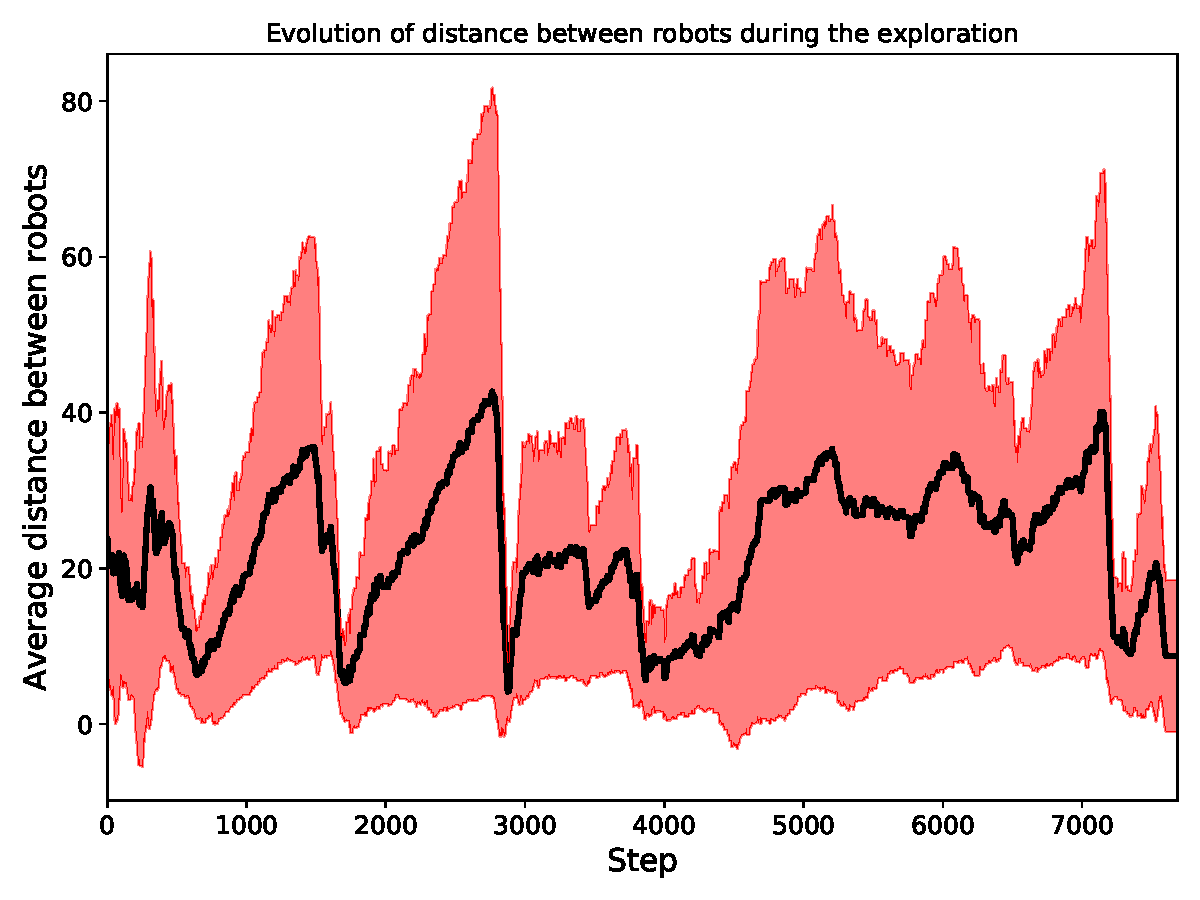
\includegraphics[width=.47\linewidth]{images/gamma_results/low_alpha/dinstance_simulation_gamma_0_32_simid_0}
	}
	\hfill
	\subfloat[Evoluzione della distanza media tra gli agenti con un valore di $\gamma$ pari a 0.65.\label{sfig:gammaSim0.65}]{
		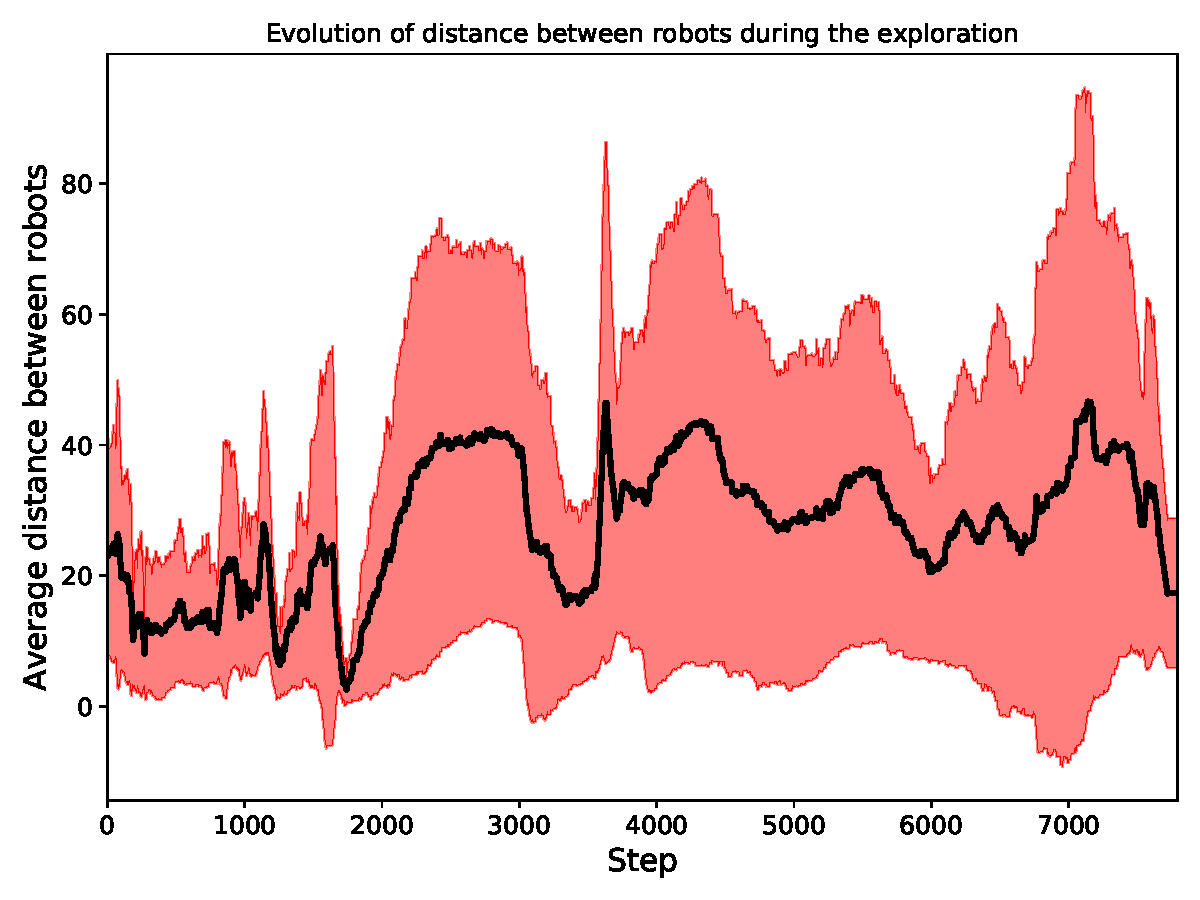
\includegraphics[width=.47\linewidth]{images/gamma_results/low_alpha/dinstance_simulation_gamma_0_65_simid_0}
	}
	\caption{Sull'asse delle \textit{x} si trova il tempo, in termini di \textit{step}, impiegato per l'esplorazione della mappa, mentre sull'asse delle \textit{y} la distanza media tra gli agenti.}
	\label{fig:gammaSim}
\end{figure}

\subsection{Analisi con valore di $\alpha$ alto}
\label{subsec:gammaahigh}
Come in precedenza, le prime analisi effettuate si sono concentrate sulla distribuzione delle distanze medie.
In Figura \ref{fig:gammaHDistr} sono rappresentate le due distribuzioni per i valori di $\gamma$ considerati in precedenza; si può notare che con valori alti di $\alpha$, l'andamento della distribuzione si sia invertita rispetto al caso precedente: per un valore pari a 0.32 (Figura \ref{sfig:gammaHDistr0.32}) la distribuzione sembra essere più “liscia”, invece per un valore pari a 0.65 (Figura \ref{sfig:gammaHDistr0.65}) o superiore sembra infittirsi per alcuni valori di distanza.
\begin{figure}
	\subfloat[Distribuzione della distanza media mantenuta dai robot con un valore di $\gamma$ pari a 0.32.\label{sfig:gammaHDistr0.32}]{
		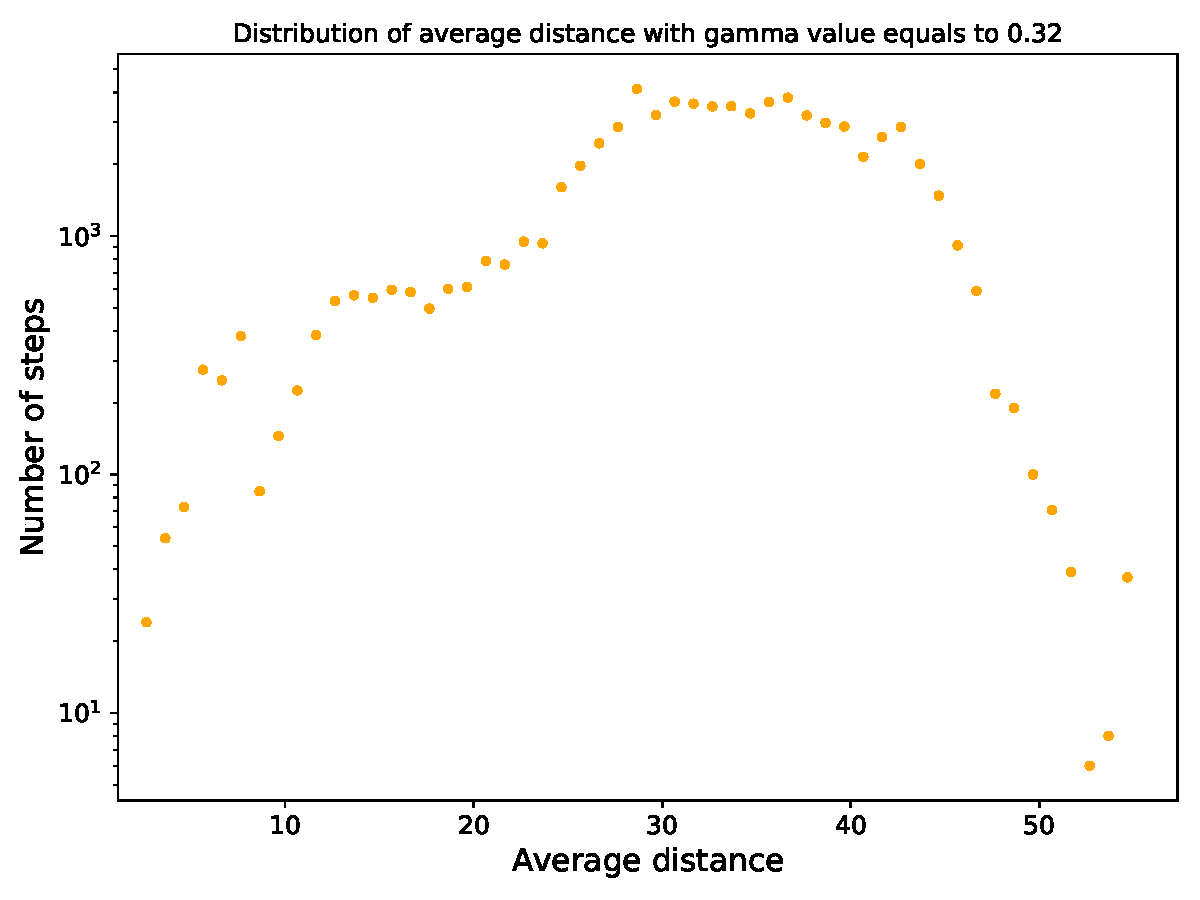
\includegraphics[width=.47\linewidth]{images/gamma_results/high_alpha/distribution_distance_gamma_0_32}
	}
	\hfill
	\subfloat[Distribuzione della distanza media mantenuta dai robot con un valore di $\gamma$ pari a 0.65.\label{sfig:gammaHDistr0.65}]{
		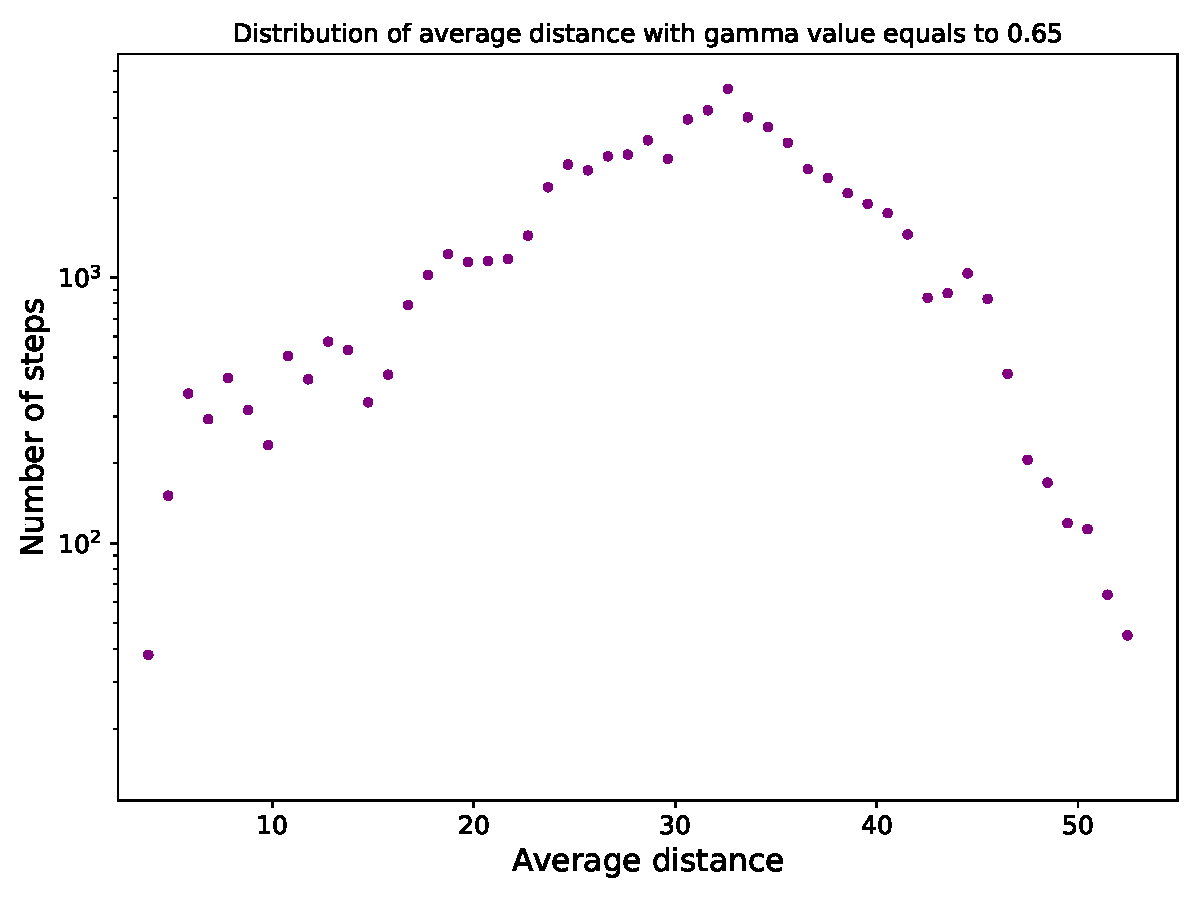
\includegraphics[width=.47\linewidth]{images/gamma_results/high_alpha/distribution_distance_gamma_0_65}
	}
	\caption{Distribuzione della distanza media mantenuta dai robot al variare del valore di $\gamma$, per valutare la distribuzione si è conteggiato in quanti \textit{step} i robot hanno presentato tale distanza, il numero di \textit{bin} per produrre la distribuzione è pari alla differenza tra la distanza minima e massima presente durante la simulazione, tale valore è stato poi arrotondato. Infine si noti che l'asse delle \textit{y} è a scala logaritmica.}
	\label{fig:gammaHDistr}
\end{figure}
Ancora una volta si è deciso di andare a confrontare tutte le distribuzioni dei valori del parametro analizzati, i risultati sono mostrati in Figura \ref{fig:gammaHComparison}.
Come si può notare, al contrario del caso precedente, per valori pari a 0.65 o 1 si notano dei “picchi” significativi e anche per valori più bassi (0.1 e 0.32) si nota come i robot mantengano una distanza media maggiore; tale risultato sembra contraddire quello detto in precedenza.\\
Per analizzare meglio questi risultati e introdurli nel quadro complessivo, bisogna considerare che non è solo $\gamma$ (come avveniva di fatto precedentemente) ad influire sulla scelta della cella obiettivo e degli spostamenti del robot, ma risulta essere vincolante anche il costo del cammino. 
Poiché il parametro $\alpha$ influisce significativamente e con una magnitudo molto maggiore rispetto all'utilità e priorità della cella nella scelta del bersaglio, il parametro $\gamma$ passa in secondo piano e influisce solo in maniera marginale sulla scelta. Ciò va ad inficiare la distanza tra i robot, poiché tali scelte non vengono più effettuate dando grande importanza all'utilità della cella quanto al tempo necessario per raggiungerla.
\begin{figure}
	\centering
	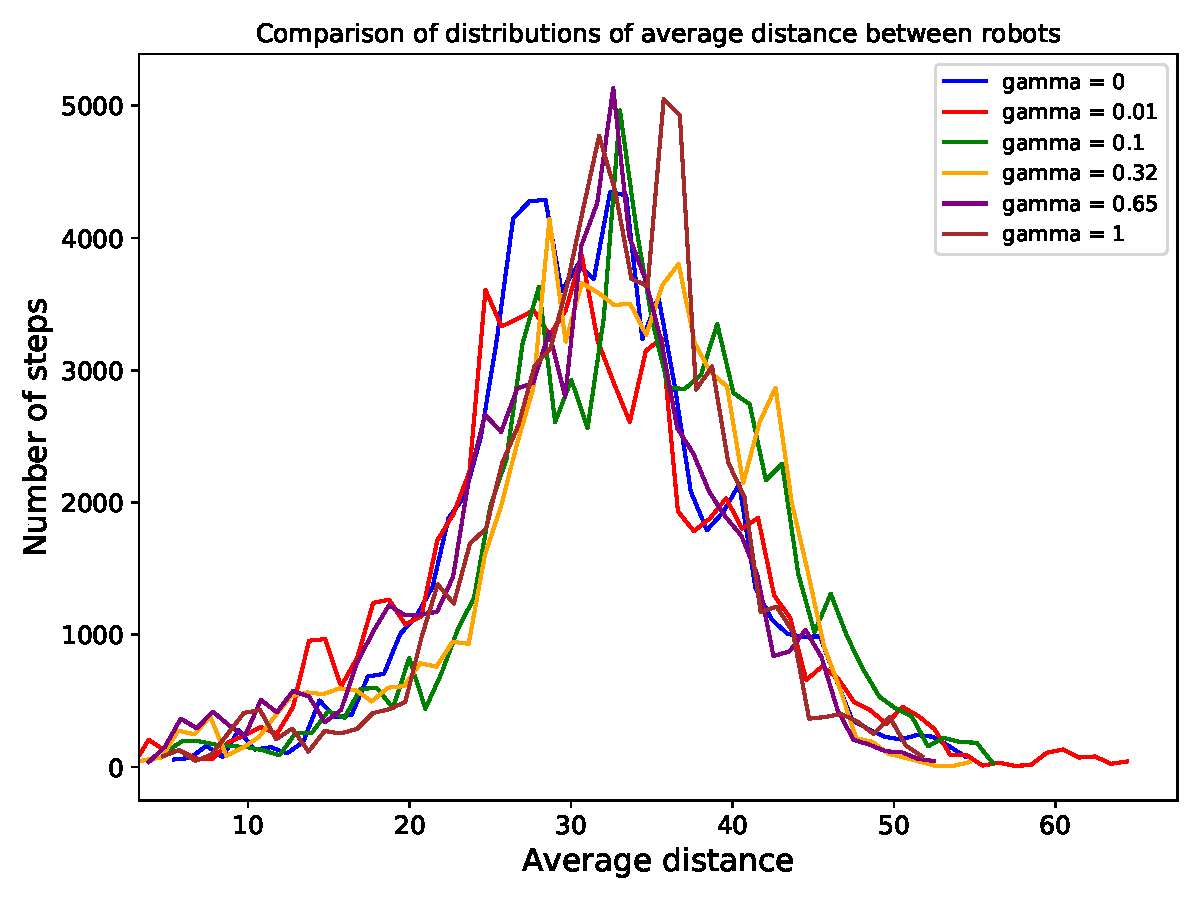
\includegraphics[width=0.9\linewidth]{images/gamma_results/high_alpha/comparison}
	\caption{Grafico che riassume tutte le distribuzioni di distanze medie durante le simulazioni per ogni valore di $\gamma$, si noti che l'asse delle \textit{y} non è più logaritmico.}
	\label{fig:gammaHComparison}
\end{figure}
Come ulteriore conferma di tale affermazione, si può notare come durante la singola simulazione non si presentino più quelle situazioni in cui la distanza tra i robot decresce significativamente a causa della segnalazione da parte dei feriti. Solo durante le fasi finali dell'esplorazione la distanza tra essi alle volte diminuisce.
Al fine di evitare che i feriti vengano di fatto ignorati, è stata implementata una seconda tecnica di prioritizzazione delle celle che, al posto di utilizzare un valore fisso stabilito a priori, utilizza un valore dipendente da $\alpha$; i risultati di tale metodo, discusso nella Sotto-sezione \ref{Ferito} saranno discussi tra breve.
L'evolversi delle distanze è rappresentato in Figura \ref{fig:gammaHSim}
\begin{figure}
	\subfloat[Evoluzione della distanza media tra gli agenti con un valore di $\gamma$ pari a 0.32.]{
		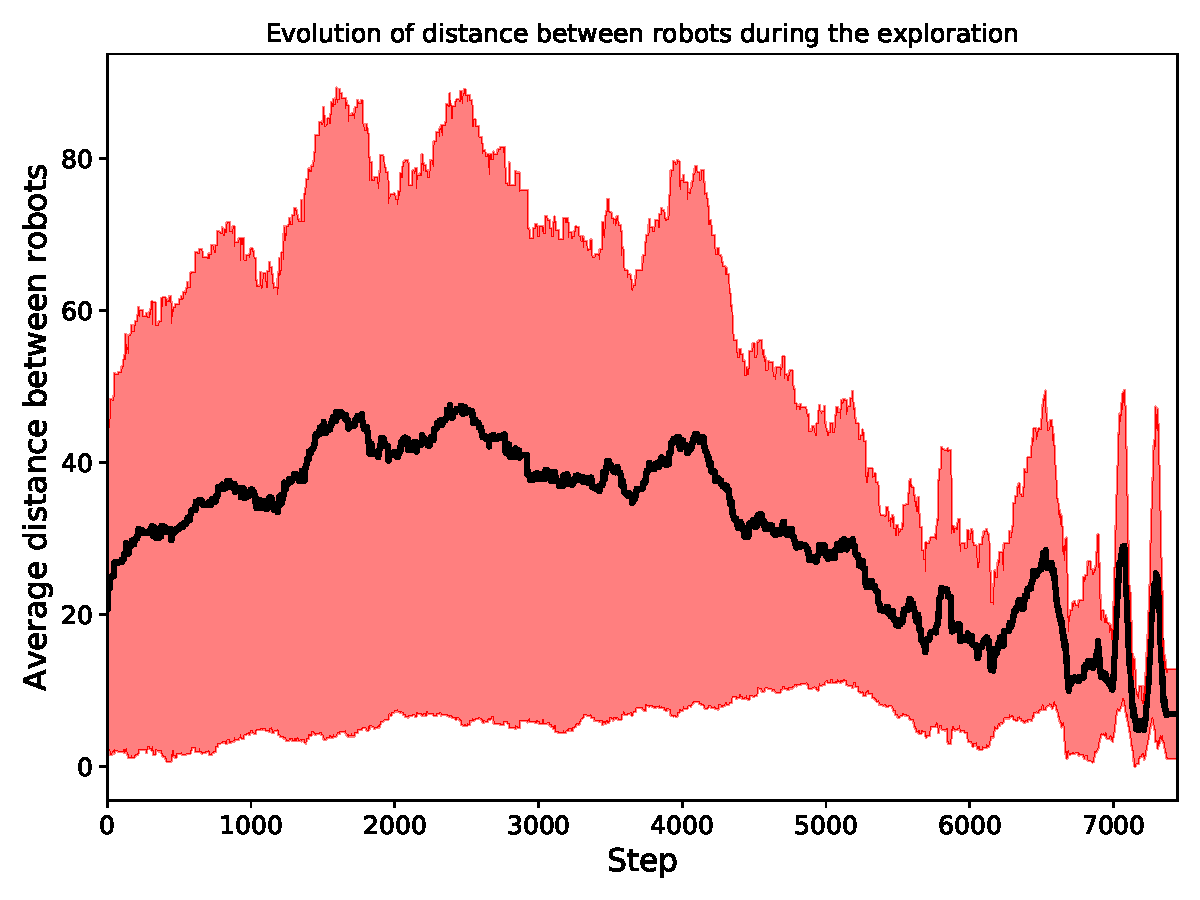
\includegraphics[width=.47\linewidth]{images/gamma_results/high_alpha/dinstance_simulation_gamma_0_32_simid_0}
	}
	\hfill
	\subfloat[Evoluzione della distanza media tra gli agenti con un valore di $\gamma$ pari a 0.65.]{
		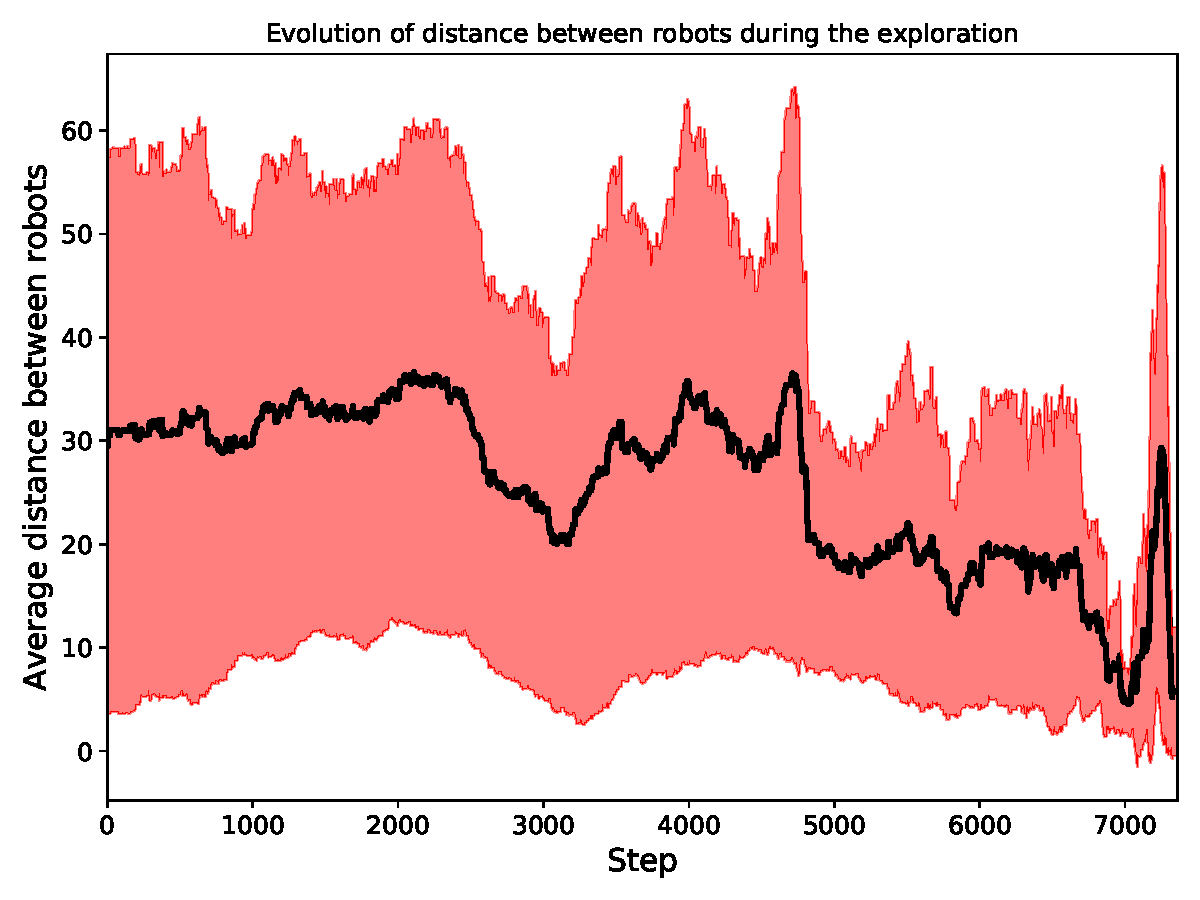
\includegraphics[width=.47\linewidth]{images/gamma_results/high_alpha/dinstance_simulation_gamma_0_65_simid_4}
	}
	\caption{Sull'asse delle \textit{x} si trova il tempo, in termini di \textit{step}, impiegato per l'esplorazione della mappa, mentre sull'asse delle \textit{y} la distanza media tra gli agenti.}
	\label{fig:gammaHSim}
\end{figure}
\subsection{Considerazioni conclusive}
In questo breve sunto, si vogliono evidenziare alcune differenze tra come opera il parametro $\gamma$ rispetto al valore di $\alpha$.
In particolare, si è notato come per valori di $\alpha$ bassi è effettivamente il parametro $\gamma$ ad influire sulla distanza tra i robot portando questi a scegliere le celle con utilità maggiore (poiché il peso influisce in maniera poco significativa) e quindi scegliendo le celle viste da meno robot (poiché sono quelle che hanno subito meno riduzioni di utilità).
In aggiunta, si evidenzia come per valori di $\alpha$ bassi i robot tenderanno a muoversi tutti verso la zona segnalata da un ferito nel momento in cui questi segnalano la loro presenza; al contempo, tale effetto sembra più marginale nel momento in cui $\alpha$ aumenta.
Nonostante queste considerazioni, si nota comunque come per valori di $\gamma$ elevati gli agenti, in entrambi i casi, tendono a rimanere più distanti rispetto a valori bassi (si tenga presente che i “picchi” per $\alpha$ elevati sono presenti per valori di distanza minori).
Ancora una volta, tale fenomeno è dovuto al fatto che quando il costo del cammino è maggiormente significativo nel calcolo dell'\textit{info-gain} diventa il principale parametro che delinea la scelta e quindi riducendo l'effetto dell'utilità delle celle e di conseguenza l'influenza del parametro $\gamma$.
\todo{test e parlare del metodo di priorità che si basa su alpha}